% !TeX root = ../libro.tex
% !TeX encoding = utf8

\chapter{Conceptos previos}

Este capítulo tiene el objetivo de introduccir los conceptos básicos utilizados en esta primera parte del proyecto. Dichos conceptos se han obtenido de las referencias \cite{MorseTh1}, \cite{MorseTh2} y \cite{Triangulacion}, junto con el conocimiento adquirido de las asignaturas de Topología II y Variedades Diferenciables.

\begin{definicion} Una \textbf{variedad topológica} 2-dimensional es un espacio de Hausdorff localmente Euclídeo que verifica el segundo axioma de numerabilidad, es decir, su topología tiene una base numerable.
\end{definicion}

\begin{definicion} Un \textbf{embebimiento o encaje} es una aplicación continua e inyectiva de un espacio topológico en otro que es un homeomorfismo sobre la imagen dotada por la topología inducida.
\end{definicion}

\begin{definicion} Un \textbf{sistema coordenado} (o carta) sobre $S$ es un embebimiento $h : \mathbb{R}^2 \rightarrow S$.
\end{definicion}

\begin{figure}[h]
  	\centering
  	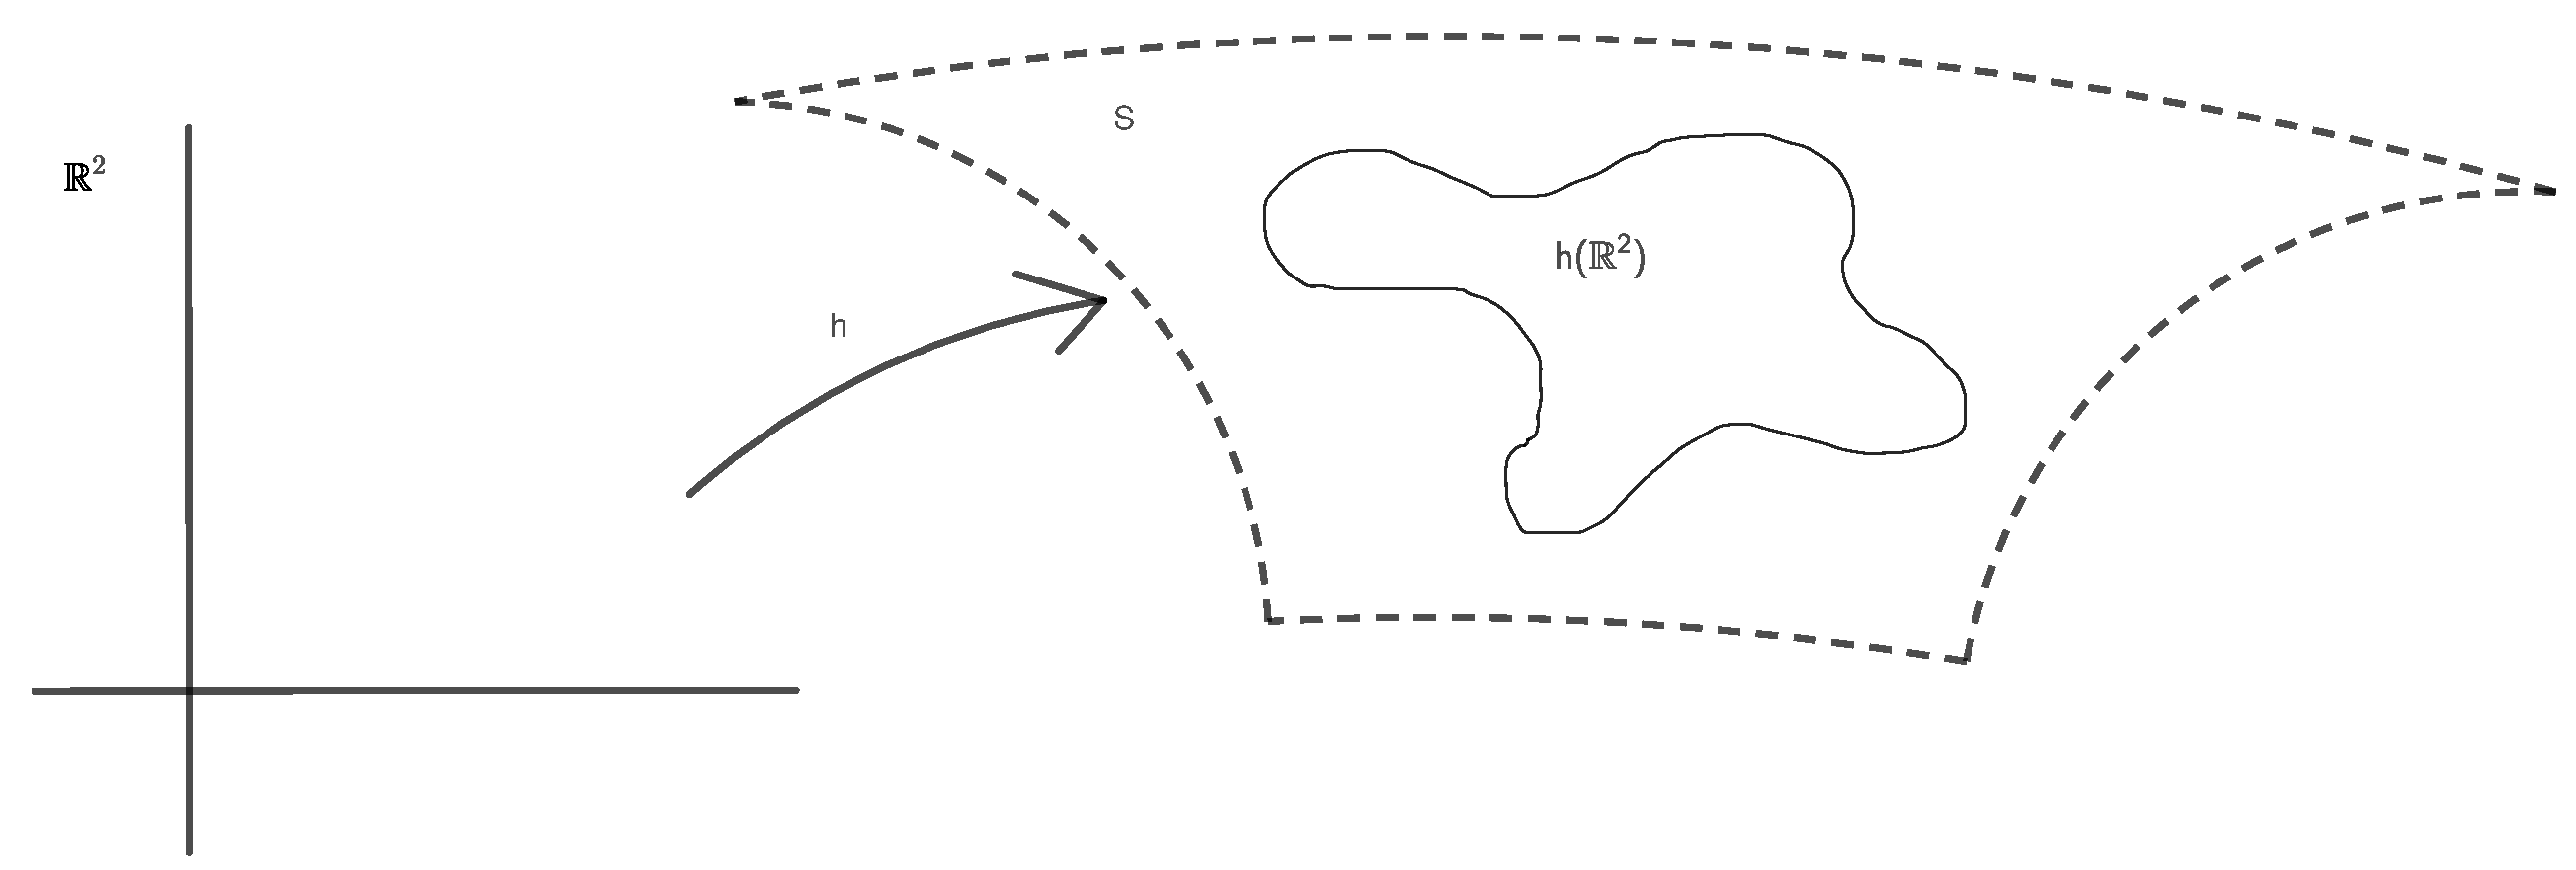
\includegraphics[width=0.7\textwidth]{ejemplo_carta}
	\caption{Ejemplo de carta.}
  	\label{fig:ejemplo_carta}
\end{figure}

\begin{definicion} Sea $S$ un espacio topológico Hausdorff, un \textbf{atlas} diferenciable $2$-dimensional sobre $S$ es una familia de cartas $E=\{h_i\}_{i\in \Lambda}$ verificando:
	\begin{enumerate}
		\item $\{h_i(\mathbb{R}^2)\}_{i\in \Lambda}$ es un recubrimiento abierto de $S$.
		\item Si $h_i(\mathbb{R}^2) \cap h_j(\mathbb{R}^2) \neq \varnothing$ entonces $h_j^{-1} \circ h_i:h_i^{-1}(h_i(\mathbb{R}^2)\cap h_j(\mathbb{R}^2)) \rightarrow h_j^{-1}(h_i(\mathbb{R}^2)\cap h_j(\mathbb{R}^2))$ es un difeomorfismo.
	\end{enumerate}
\end{definicion}

\begin{definicion} Sea $S$ un espacio topológico Hausdorff, una \textbf{estructura diferenciable} $2$-dimensional sobre $S$ es un atlas diferenciable maximal.
\end{definicion}

\begin{definicion} Una \textbf{variedad diferenciable} 2-dimensional es una variedad topológica $2$-dimensional $S$ junto con una estructura diferenciable $E$, es decir, el par $(S, E)$.
\end{definicion}

\begin{definicion} Una aplicación $f: N \rightarrow M$ entre las variedades diferenciables $N$ y $M$ se dice que es \textbf{diferenciable} si la composición con las cartas de ambas estructuras diferenciables es diferenciable en el sentido real, es decir, $\forall \phi \in E_N$, $\forall \psi \in E_M$ se tiene que $\psi^{-1} \circ f \circ \phi$ es diferenciable.
\end{definicion}

\begin{definicion} Una \textbf{inmersión} es una aplicación diferenciable entre variedades diferenciables cuya diferencial es inyectiva en todo punto.
\end{definicion}

\begin{definicion} Una n-celda $n \in \N$, en un espacio topológico $X$, es una aplicación continua $f: \overline{B}^n \rightarrow X$ tal que, si llamamos $C=f(B^n)$, la aplicación $f|_{B^n}:B^n \rightarrow C$ es un homeomorfismo (donde $B^n$ es la bola unidad abierta en $\R^n$ y $\overline{B}^n$ la cerrada). Si $X$ es una variedad diferenciable y $f$ es diferenciable (es decir, extiende diferenciablemente más allá de $\overline{B}^n$), la celda se dirá diferenciable.\\
\\Al conjunto $f(\partial B^n)=f(S^{n-1})$ se le llama caras borde de la celda (lados si $n=2$, vértices si $n=1$), mientras que al conjunto $C$ se le refiere como el interior de la celda. Es común identificar la celda con el conjunto $C$ si ello no conlleva a ambigüedad.
\end{definicion}

\begin{definicion} Una \textbf{triangulación diferenciable} de una variedad diferenciable $X$ es un conjunto de celdas diferenciables con interiores disjuntos dos a dos y cuya unión es $X$.
\end{definicion}

\begin{definicion} Sean $f$ y $g$ homeomorfismos entre los espacios topológicos $X$ e $Y$. Una \textbf{isotopía} es una homotopía que deforma $f$ en $g$, $H: X \times [0,1] \rightarrow Y$, y que satisface:
	\begin{enumerate}
		\item $H(\cdot, t) : X \rightarrow Y$ es un homeomorfismo $\forall t \in [0,1]$.
		\item $H(p, 0) = f(p)$, $H(p, 1) = g(p)$ $\forall p \in X$.
	\end{enumerate}
\end{definicion}

\begin{definicion} Dos embebimientos $f,g : N \rightarrow M$ de una variedad $N$ en otra $M$ se dicen \textbf{isotópicos} si existe $H: N \times [0,1] \rightarrow M$ aplicación continua tal que:
	\begin{enumerate}
		\item $H(\cdot, t) : N \rightarrow M$ es un embebimiento $\forall t \in [0,1]$.
		\item $H(p, 0) = f(p)$, $H(p, 1) = g(p)$ $\forall p \in N$.
	\end{enumerate}
\end{definicion}

\begin{definicion} Sea $M$ una variedad diferenciable y $f: M \rightarrow \R$ una función diferenciable en $M$. Un punto $p \in M$ se dice que es un $\textbf{punto crítico}$ de $f$ si $Df(p) = 0$ en $T_pM$. A su imagen por $f$, $f(p)$, se le dice $\textbf{valor crítico}$ de $f$.
\end{definicion}

\begin{definicion} Sea $M$ una variedad diferenciable y $f: M \rightarrow \R$ una función diferenciable en $M$. Un punto crítico $p \in M$ se dice que es $\textbf{no degenerado}$ si $H_\phi(f)(p)$ es regular para cualquier parametrización $\phi$ centrada en $p$, donde $H_\phi(f)=H(f \circ \phi)$ es la matriz Hessiana de $f \circ \phi$.\\ 
\\ El $\textbf{índice}$ de dicho punto es la dimensión del mayor subespacio de $T_pM$ donde $H_\phi(f)$ es definida negativa. No depende de $\phi$ por la regla de Sylvester, ya que $H$ para otra parametrización $\psi$ cumple $H_\psi(f) = J^t(\theta) H_\phi(f) J(\theta)$, con $\theta$ el cambio de coordenadas y $J$ la matriz Jacobiana.
\end{definicion}

\begin{definicion} Sea $f:M \to \R$ función diferenciable, con $M$ una variedad, se dice que es una $\textbf{función de Morse}$ si todos sus puntos críticos son no degenerados.
\end{definicion}

\newpage
\begin{definicion} Sea $f$ una función de Morse en una superficie diferenciable $S$, dados $a < b$ valores regulares de $f$ en $\R$ definimos:
	\begin{itemize}
		\item $V(a) = f^{-1}(a)$, se suele referir como una curva de nivel $f$.
		\item $M(a) = f^{-1}((-\infty, a])$, el conjunto que hay ``debajo'' de la curva de nivel para el valor regular $a$.
		\item $M'(a) = f^{-1}([a,\infty))$, el conjunto que hay ``encima'' de la curva de nivel para el valor regular $a$.
		\item $W(a,b) = f^{-1}([a,b])$, el conjunto contenido entre 2 curvas de nivel.
	\end{itemize}
\end{definicion}

\begin{figure}[h]
  	\centering
  	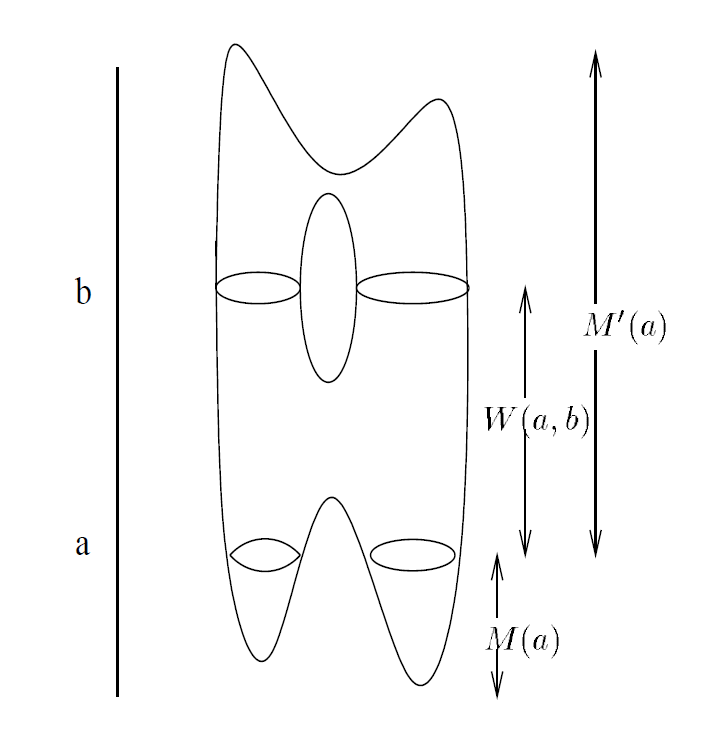
\includegraphics[width=0.4\textwidth]{niveles_morse}
  	\label{fig:niveles_morse}
\end{figure}

\begin{definicion} Una aplicación continua $f$ se dice \textbf{propia} si para todo compacto $M$, su imagen por $f^{-1}$ es compacta.
\end{definicion}

\endinput
%------------------------------------------------------------------------------------
% FIN DEL CAPÍTULO. 
%------------------------------------------------------------------------------------
